
include(`macros.m4')

%%%%%

\begin{slide}
\sltitle{Hierarchical file system}
\begin{center}
\input{img/tex/fstree.pstex_t}
\end{center}
\end{slide}

\begin{itemize}
\item A \emph{file system} is a data structure to control how data is stored and
retrieved.  Without it the stored data would have no structure, ownership, etc.
The filesystem structure provides for storing directories (folders), files,
metadata, etc.
\item Each filesystem has a specific structure type it uses, for example
\texttt{ext4} (Linux specific), \texttt{XFS} (used on Linux but coming from SGI
IRIX), \texttt{JFS} (used on Linux but came from IBM AIX), \texttt{UFS} (BSD
systems), \texttt{FAT32} (Win), \texttt{ZFS} (Solaris born, then ported to other
systems), \texttt{APFS} (macOS and iOS since 2017), etc.  A filesystem can be
either used on local or remote storage, and in case of a remote storage network
filesystem protocols like \texttt{NFS} or \texttt{AFS} are used to access the
data.  Note that these network filesystems do not define the filesystem
structure itself, they only provide for accessing existing filesystems remotely.
Each filesystem also has its limits, a largest file size or the maximum size of
the filesystem itself, for example.
\item Unix does not have A, B, C, D\dots disks as Windows and other systems.
All filesystems are mounted to a single directory hierarchy on any Unix system,
as shown on the slide where you can see the root filesystem and three other
fileystems, mounted on \texttt{/usr}, \texttt{/dev/tty}, and \texttt{/home}
directories.  You could also further mount other filesystems on directories that
are part of these non-root filesystems.
\item Each filesystem mounted to the common hierarchy may be formatted using a
different filesystem type.  However, that is largely transparent to a user
traversing the hierarchy.  There are some exceptions though.  For example,
\texttt{FAT32} does no provide user and access rights for files so those are
faked when such filesystem is mounted.
\item Upon the system boot, the root filesystem is mounted first, other
filesystems are later mounted via the \texttt{mount} command, usually from
specific startup services based on the system you use.  The startup services
sometimes use file \texttt{/etc/fstab} as a source of information about what
filesystems to mount.  You can also use \texttt{mount} manually.  To unmount a
filesystem, the \texttt{umount} command is used.
\item Some systems also provide for auto mounting where filesystems are mounted
during the first access attempt, and may be automatically unmounted after a
period of inactivity.  Such functionality is usually called an
\emph{automounter}.  See \texttt{autofs}, \texttt{automount}, or \texttt{amd}
for more information.
\end{itemize}

%%%%%

\pdfbookmark[1]{typical layout of system directories}{hier}

\begin{slide}
\sltitle{Typical layout of system directories}
\begin{tabular}{l@{\hspace{3ex}\dots\hspace{3ex}}l}
\texttt{/bin} & basic system commands\\
\texttt{/dev} & devices\\
\texttt{/etc} & configuration\\
\texttt{/lib} & basic system libraries\\
\texttt{/tmp} & public directory for temporary files\\
\texttt{/home} & root of home directories\\
\texttt{/var/adm} & administrative files (not on BSD) \\
\texttt{/usr/in{}clude} & header files for C\\
\texttt{/usr/local} & locally installed software\\
\texttt{/usr/man} & man pages\\
\texttt{/var/spool} & spool (mail, printing,...)
\end{tabular}
\end{slide}

\begin{itemize}
\item The \texttt{/bin}, \texttt{/lib}, \texttt{/sbin} directories contain
commands and libraries needed for the start of the system when only root
filesystem is mounted. The rest of the commands is located typically in
\texttt{/usr/bin}, \texttt{/usr/lib} and \texttt{/usr/sbin}.
\texttt{/usr} may be a separate file system, possibly not accessible during
system startup.
\item The \texttt{s} letter in \texttt{sbin} means ,,system'', not SUID.
It contain binaries not needed by typical user.
\item The \texttt{/usr} directory tree contains files that are not changing
while the system is running and are not dependent on given machine.
This property should make it elegible for read-only sharing. On your own
machine it will be typically read-write, though.
\item The \texttt{/lib} directory typically contains libraries needed for
programs from the root file system. If all libraries were in \texttt{/usr/lib}
and \texttt{/usr} was separate file system, a problem with mounting
\texttt{/usr} could paralyze complete system, because no program could be run.
In some systems the root file system contains base set of programs that are
statically linked. For example FreeBSD has such binaries under the
\texttt{/rescue} directories. It also has separate directories \texttt{/lib} and
\texttt{/usr/lib}.
\item The \texttt{/var} directory tree contains data that change while the
system is running and are specific for given machine.
\item There can be differences in directory layout found between installations
of the same operating system.
\item The \texttt{hier(7)} manual page on FreeBSD and Linuxu describes directory
hierarchy on these systems. Solaris uses \texttt{filesystem(5)}.
\end{itemize}

%%%%%

\begin{slide}
\sltitle{Peripheral device access}
\begin{itemize}
\item The \texttt{/dev} directory contains special device files.
A process opens special file via \texttt{open()} and communicates with the
device via \texttt{read()}, \texttt{write()}, \texttt{ioctl()}, etc.
\item special files are divided into:
    \begin{itemize2}
    \item \emsl{character} \dots{} data is transferred directly between process
    and device driver, e.g. serial ports
    \item \emsl{block} \dots{} data is passed through system cache
    (buffer cache) in blocks of given size, e.g. disks
    \end{itemize2}
\item special device identifies concrete device with two numbers
    \begin{itemize2}
    \item \emsl{major} \dots{} number of device driver in the kernel
    \item \emsl{minor} \dots{} number within single device driver
    \end{itemize2}
\end{itemize}
\end{slide}

\begin{itemize}
\item The cache speeds up operations with peripheral devices. When reading the
data is searched in the buffer first. When not present there, they are being
read from disk. For the next read they are already available in the buffer.
For writing the data is stored into a buffer that is written to the disk later.
It is possible to force immediate write to disk. In today's systems the cache is
not a standalone structure, rather it is part of virtual memory system.
\item Disks in Unix are usually accessible using both character and block
interface. The former is used by \texttt{mkfs} when creating the file system and
also by \texttt{fsck} when performing file system consistency check.
The latter is used for normal reads and writes. Some systems (FreeBSD) do not
have block devices under \texttt{/dev}.
\item In the past, the contents of the \texttt{/dev} directory had to be
refreshed by a shell script (\texttt{MAKEDEV}) or by hand whenever hardware
configuration changed. Today most of the systems populate the directory on the
fly as kernel detects addition or removal of hardware components
(see \emph{devfs} on page \pageref{DEVFS}).
\item Immediate write to disk can be forced by using the \texttt{O\_DIRECT}
command via the \texttt{fcntl} system call.
\end{itemize}

%%%%%

\begin{slide}
\sltitle{Physical layout of file system}
\begin{itemize}
\item \emsl{filesystem} can be created on:
    \begin{itemize2}
    \item \emsl{partition} -- part of disk, one disk can have multiple
    partitions
    \item \emsl{logick�m volume} -- can be used to connect multiple partitions
    (that can reside on distinct disks) into one file system.
    \end{itemize2}
\item more choices: striping, mirroring, RAID
\end{itemize}
\begin{center}
\input{img/tex/partitions.pstex_t}
\end{center}
\end{slide}

\begin{itemize}
\item the expression \emsl{file system} has multiple meanings:
    \begin{itemize}
    \item one file system, i.e. what the \texttt{mkfs} command creates
    \item whole hierarchy of file systems (the output of the
    \texttt{mount} command)
    \item way of organizing given file system and its corresponding kernel
    module that manipulates the data (UFS2, Ext3, XFS, ...)
    \end{itemize}
\item striping means that data blocks that follow each other are stored in
parallel on distinct drives, boosting the speed of read operations.
\item mirroring stores copies of data to multiple disks to provide redundancy.
\item parity disks: data is saved to e.g. 2 drives and the \nth{3} drive is used
for storing XOR value of the first two. If any single disk fails, the data can
be reconstructed.
\item individual RAID (Redundant Array of Inexpensive Disks) levels include
striping, mirroring and parity disks.
\item The terminology has to be used with care. For example what is meant by
\emph{partition} in the DOS world, is being called \emph{slice} in BSD.
There the partitions are defined within one slice and the file systems are
created therein.
\item ZFS combines both volume manager and file system. It was ported from
Solaris to BSD systems.
\end{itemize}

%%%%%

\pdfbookmark[1]{UNIX System V file system}{sysVfs}

\begin{slide}
\sltitle{The \texttt{s5} file system organization}
\begin{center}
\begin{picture}(0,0)%
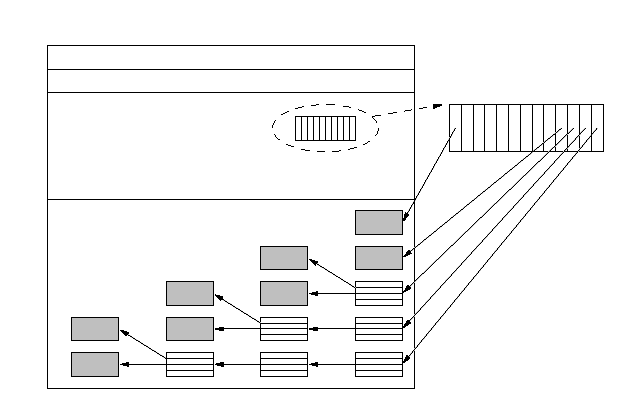
\includegraphics{img/tex/s5}%
\end{picture}%
\setlength{\unitlength}{4144sp}%
%
\begingroup\makeatletter\ifx\SetFigFont\undefined%
\gdef\SetFigFont#1#2#3#4#5{%
  \reset@font\fontsize{#1}{#2pt}%
  \fontfamily{#3}\fontseries{#4}\fontshape{#5}%
  \selectfont}%
\fi\endgroup%
\begin{picture}(4467,2832)(46,-2053)
\put(3331,164){\makebox(0,0)[lb]{\smash{\SetFigFont{10}{12.0}{\sfdefault}{\mddefault}{\updefault}{\color[rgb]{0,0,0}0}%
}}}
\put(4141,164){\makebox(0,0)[lb]{\smash{\SetFigFont{10}{12.0}{\sfdefault}{\mddefault}{\updefault}{\color[rgb]{0,0,0}9}%
}}}
\put(4366,164){\makebox(0,0)[lb]{\smash{\SetFigFont{10}{12.0}{\sfdefault}{\mddefault}{\updefault}{\color[rgb]{0,0,0}12}%
}}}
\put(1336,254){\makebox(0,0)[lb]{\smash{\SetFigFont{10}{12.0}{\sfdefault}{\mddefault}{\updefault}{\color[rgb]{0,0,0}superblock}%
}}}
\put(361, 29){\makebox(0,0)[lb]{\smash{\SetFigFont{10}{12.0}{\sfdefault}{\mddefault}{\updefault}{\color[rgb]{0,0,0}i-node area}%
}}}
\put(361,-781){\makebox(0,0)[lb]{\smash{\SetFigFont{10}{12.0}{\sfdefault}{\mddefault}{\updefault}{\color[rgb]{0,0,0}data block area}%
}}}
\put( 46,659){\makebox(0,0)[lb]{\smash{\SetFigFont{10}{12.0}{\sfdefault}{\mddefault}{\updefault}{\color[rgb]{0,0,0}block number}%
}}}
\put( 91,434){\makebox(0,0)[lb]{\smash{\SetFigFont{10}{12.0}{\sfdefault}{\mddefault}{\updefault}{\color[rgb]{0,0,0}0}%
}}}
\put( 91,254){\makebox(0,0)[lb]{\smash{\SetFigFont{10}{12.0}{\sfdefault}{\mddefault}{\updefault}{\color[rgb]{0,0,0}1}%
}}}
\put( 91, 74){\makebox(0,0)[lb]{\smash{\SetFigFont{10}{12.0}{\sfdefault}{\mddefault}{\updefault}{\color[rgb]{0,0,0}2}%
}}}
\put(113,-91){\rotatebox{270.0}{\makebox(0,0)[lb]{\smash{\SetFigFont{14}{16.8}{\sfdefault}{\mddefault}{\updefault}{\color[rgb]{0,0,0}...}%
}}}}
\put(758,434){\makebox(0,0)[lb]{\smash{\SetFigFont{10}{12.0}{\sfdefault}{\mddefault}{\updefault}{\color[rgb]{0,0,0}boot block}%
}}}
\end{picture}

\end{center}
\end{slide}

\begin{itemize}
\item the original UNIX file system used by default until System V Release 3;
used in BSD until 4.1
\item properties:
    \begin{itemize}
    \item 512, 1024 or 2048 byte blocks
    \item single (non-duplicated) superblock
    \item data area divided into \emph{i-node} and \emph{data block} parts
    \item with 1024 byte blocks the theoretical size is over 16 GB
    \end{itemize}
\item \emph{boot block} -- for OS boot loader
\item \emph{superblock} -- basic information about the file system: number of
blocks for i-nodes, number of file system block, list of feee blocks (continues
in the free block area), list of free i-nodes (after it is exhausted the i-node
table is searched), locks for the lists of free data blocks and i-nodes,
modification flag (used for checking whether the file system was correctly
unmounted), time of the last update, device information.
\item \emph{i-node} -- file type, access rights, owner, group, times of last
access, modification and i-node modification, number of references, file size,
10 pointers to data blocks and 3 indirect pointers. Note that the time of file
creation is not stored.
\item maximal file system size: 2113674 blocks, .i.e approximately 1 GB when
using 512 byte blocks
\item file names -- max. 14 characters (14 + 2 = 16, .i.e. power of 2 and
therefore seamless storage of directory entries into blocks)
\item the file system was able to utilize the disks only to approximately 2\%
and read operations were able to fetch tens of kilobytes per second.
\item for comparison -- MS-DOS 2.0 from 1983 supported only FAT12, with maximal
file system size of 16 MB. The maximal size up to 2 GB was made possible only in
version 4.0 (1988); this version also introduced disk caches, i.e. feature that
UNIX has had since its inception in 1970.
\end{itemize}

%%%%%

\begin{slide}
\sltitle{Directory structure navigation}
\begin{center}
\input{img/tex/nav_dir.pstex_t}
\end{center}
\end{slide}

\begin{itemize}
\item if a path begins with '\texttt{/}', the navigation starts in the root
directory, otherwise it starts in the working directory of given process.
\item the i-node number of root directory is typically 2. 0 is reserved for
empty i-node and 1 used to be a file into which bad blocks were inserted to
avoid them being used.

\item path that has multiple consecutive slashes is still valid, i.e.
\texttt{///a///b///c} is equivalent to \texttt{/a/b/c}.
\end{itemize}


%%%%%

\pdfbookmark[1]{links and their properties}{links}

\begin{slide}
\sltitle{Links}
\begin{center}
\begin{picture}(0,0)%
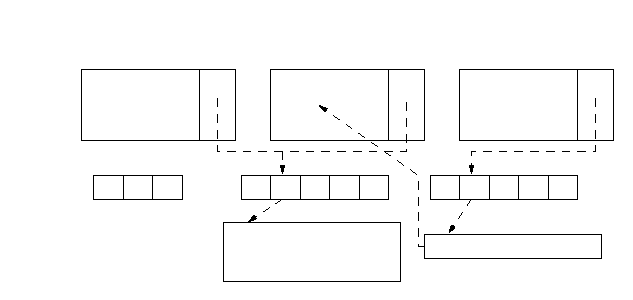
\includegraphics{img/tex/links}%
\end{picture}%
\setlength{\unitlength}{4144sp}%
%
\begingroup\makeatletter\ifx\SetFigFont\undefined%
\gdef\SetFigFont#1#2#3#4#5{%
  \reset@font\fontsize{#1}{#2pt}%
  \fontfamily{#3}\fontseries{#4}\fontshape{#5}%
  \selectfont}%
\fi\endgroup%
\begin{picture}(4557,2022)(46,-1333)
\put(721,-646){\makebox(0,0)[lb]{\smash{\SetFigFont{10}{12.0}{\sfdefault}{\mddefault}{\updefault}{\color[rgb]{0,0,0}0}%
}}}
\put(2026,-646){\makebox(0,0)[lb]{\smash{\SetFigFont{10}{12.0}{\sfdefault}{\mddefault}{\updefault}{\color[rgb]{0,0,0}20}%
}}}
\put(3466,-646){\makebox(0,0)[lb]{\smash{\SetFigFont{10}{12.0}{\sfdefault}{\mddefault}{\updefault}{\color[rgb]{0,0,0}31}%
}}}
\put(3241,-1096){\makebox(0,0)[lb]{\smash{\SetFigFont{10}{12.0}{\ttdefault}{\mddefault}{\updefault}{\color[rgb]{0,0,0}../etc/passwd}%
}}}
\put(631,119){\makebox(0,0)[lb]{\smash{\SetFigFont{10}{12.0}{\ttdefault}{\mddefault}{\updefault}{\color[rgb]{0,0,0}password}%
}}}
\put(1486,119){\makebox(0,0)[lb]{\smash{\SetFigFont{10}{12.0}{\sfdefault}{\mddefault}{\updefault}{\color[rgb]{0,0,0}20}%
}}}
\put(631,-151){\makebox(0,0)[lb]{\smash{\SetFigFont{14}{16.8}{\sfdefault}{\mddefault}{\updefault}{\color[rgb]{0,0,0}...}%
}}}
\put(2926,119){\makebox(0,0)[lb]{\smash{\SetFigFont{10}{12.0}{\sfdefault}{\mddefault}{\updefault}{\color[rgb]{0,0,0}20}%
}}}
\put(2071,119){\makebox(0,0)[lb]{\smash{\SetFigFont{10}{12.0}{\ttdefault}{\mddefault}{\updefault}{\color[rgb]{0,0,0}passwd}%
}}}
\put(2071,-151){\makebox(0,0)[lb]{\smash{\SetFigFont{14}{16.8}{\sfdefault}{\mddefault}{\updefault}{\color[rgb]{0,0,0}...}%
}}}
\put(4366,119){\makebox(0,0)[lb]{\smash{\SetFigFont{10}{12.0}{\sfdefault}{\mddefault}{\updefault}{\color[rgb]{0,0,0}31}%
}}}
\put(3511,119){\makebox(0,0)[lb]{\smash{\SetFigFont{10}{12.0}{\ttdefault}{\mddefault}{\updefault}{\color[rgb]{0,0,0}passwd}%
}}}
\put(3511,-151){\makebox(0,0)[lb]{\smash{\SetFigFont{14}{16.8}{\sfdefault}{\mddefault}{\updefault}{\color[rgb]{0,0,0}...}%
}}}
\put(1441,-646){\makebox(0,0)[lb]{\smash{\SetFigFont{14}{16.8}{\sfdefault}{\mddefault}{\updefault}{\color[rgb]{0,0,0}...}%
}}}
\put(2926,-646){\makebox(0,0)[lb]{\smash{\SetFigFont{14}{16.8}{\sfdefault}{\mddefault}{\updefault}{\color[rgb]{0,0,0}...}%
}}}
\put(1711,-1051){\makebox(0,0)[lb]{\smash{\SetFigFont{10}{12.0}{\ttdefault}{\mddefault}{\updefault}{\color[rgb]{0,0,0}root:x:0:...}%
}}}
\put(811,569){\makebox(0,0)[lb]{\smash{\SetFigFont{10}{12.0}{\sfdefault}{\mddefault}{\updefault}{\color[rgb]{0,0,0}hard link}%
}}}
\put(901,389){\makebox(0,0)[lb]{\smash{\SetFigFont{10}{12.0}{\ttdefault}{\mddefault}{\updefault}{\color[rgb]{0,0,0}/var}%
}}}
\put(2251,569){\makebox(0,0)[lb]{\smash{\SetFigFont{10}{12.0}{\sfdefault}{\mddefault}{\updefault}{\color[rgb]{0,0,0}original}%
}}}
\put(2341,389){\makebox(0,0)[lb]{\smash{\SetFigFont{10}{12.0}{\ttdefault}{\mddefault}{\updefault}{\color[rgb]{0,0,0}/etc}%
}}}
\put(3466,569){\makebox(0,0)[lb]{\smash{\SetFigFont{10}{12.0}{\sfdefault}{\mddefault}{\updefault}{\color[rgb]{0,0,0}symbolic link}%
}}}
\put(3781,389){\makebox(0,0)[lb]{\smash{\SetFigFont{10}{12.0}{\ttdefault}{\mddefault}{\updefault}{\color[rgb]{0,0,0}/usr}%
}}}
\put( 46,-646){\makebox(0,0)[lb]{\smash{\SetFigFont{10}{12.0}{\sfdefault}{\mddefault}{\updefault}{\color[rgb]{0,0,0}i-nodes}%
}}}
\put( 46,-1141){\makebox(0,0)[lb]{\smash{\SetFigFont{10}{12.0}{\sfdefault}{\mddefault}{\updefault}{\color[rgb]{0,0,0}data}%
}}}
\end{picture}

\end{center}

Hard links can be created within one (logical) file system.
\end{slide}

\begin{itemize}
\item what is ``normally'' visible in directory listings are hard links.
W.r.t. files there are \emsl{only} hardlink a symlinks.

\begin{description}
\item[hardlink]~

    \begin{itemize}
    \item reference to the same i-node
    \item actually second name of a file
    \item no difference between original and hard link
    \item can be created only within one file system
    \item not possible to create for directories
    \end{itemize}
\item [symbolic link (symlink, softlink)]~

    \begin{itemize}
    \item only reference to the real path of file of different type
    (it is marked as '\texttt{l}' in the \texttt{ls -l} output), i.e. the type
    of symbolic differs from ordinary file. Its data contain a simple string
    -- name of the path, either relative or absolute.
    \item different behavior for original and symlink (e.g. upon unlink)
    \item watch out for relative and absolute paths when moving symbolic link
    \item can point to directory or non-existing file
    \end{itemize}
\end{description}

\item the simplest way how to verify that two links point to the same file is to
use the \texttt{-i} option of the \texttt{ls} command, that will show the i-node
number.

\begin{verbatim}
$ ls -i /etc/passwd
172789 /etc/passwd
\end{verbatim}
\end{itemize}

%%%%%

\begin{slide}
\sltitle{File system enhancements}
\begin{itemize}
\item the goal: lower file fragmentation, reduce head moves by storing i-nodes
and data blocks closer
\item UFS (Unix File System), originally Berkeley FFS (Fast File System)
\item divided into cylinder groups, each contains:
    \begin{itemize}
    \item superblock copy
    \item cylinder group header
    \item i-node table
    \item bitmaps for free i-nodes and data blocks
    \item data blocks
    \end{itemize}
\item bloks of size 4 to � 8 kB, smaller parts stored into block fragments
\item file names up to 255 characters
\end{itemize}
\end{slide}

\begin{itemize}
\item The superblock in each cylinder group was shifted so that superblocks do
not share the same platter.
\item more file systems: UFS2, Ext3, ReiserFS, XFS, ZFS etc.
\item UFS was still 32-bit, that reflected on maximum file length and maximum
file system size. The 32-bit notation means that i-node numbers are represented
as 32 bit integers. This gives the theoretical filesystem limits.
\item journalling (XFS, Ext3, ReiserFS) -- an effort to reduce the risk of data
loss in case of crash and also to speed up the recovery after crash.
\item ZFS -- modern 128-bit file system developed in Sun Microsystems, since
Solarisu 10; also present in FreeBSD since version 7.
\end{itemize}

%%%%%

\begin{slide}
\sltitle{The development in directory entry management}
\begin{itemize}
\item maximum file name length of 14 characters was not enough
\item FFS -- up to 255 characters; each entry also contains its length
\item new file systems use B-trees for internal directory structure
representation
    \begin{itemize}
    \item considerably speeds up the work with directories that contain huge
    number of files
    \item XFS, JFS, ReiserFS, \dots
    \end{itemize}
\item UFS2 introduced backward compatible \emph{dirhash} for speeding up
the access to directories with lots of files
\end{itemize}
\end{slide}

\begin{itemize}
\item The principle of \emph{dirhash} is that after first read of a directory a
hash structure is created in memory. Subsequent directory accesses are then
comparable to the implementations using B-trees. This way an enhancement is made
without changing on-disk layout of the file system. Such enhancements cannot be
made forever, eventually on-disk format has to change or transition to another
file system is necessary.
\item small files are often stored in i-nodes, which saves disk I/O
\end{itemize}

%%%%%

\pdfbookmark[1]{Virtual File System}{VFS}

\begin{slide}
\sltitle{Virtual File System}
\begin{center}
\input{img/tex/vfs.pstex_t}
\end{center}
\end{slide}

\begin{itemize}
\item The \emph{FFS} filesystem introduced in 4.2BSD was historically the second
unix filesystem. Some manufacturers of unix system started to prefer its
considering its better performance and new features, others remained with 
\emph{s5fs} from compatibility reasons. This deepened the problem with already
insufficient interoperability between different unix systems. For some
applications neither of these filesystems was enough. Gradually the need to work
with non-unix systems started appearing, e.g. with \emph{FAT}. With growing
popularity of computer networks the demand for file sharing between systems
started to increase. This lead to the inception of distributed filesystems
-- e.g. \emph{NFS} (Network File System).
\item Given the above described situation it was just a matter of time when
fundamental changes in the filesystem infrastructure will happen to support
multiple filesystem types simultaneously. Several different implementations from
multiple manufacturers were made; in the end the de facto standard became
the \emph{VFS/vnode} architecture from Sun Microsystems. Today practically all
unix u{}nix-like systems support VFS, even though with often non-compatible
changes. VFS appeared for the first time in 1985 in Solaris 2.0;
soon it was adopted by BSD -- FFS with VFS support started to be called UFS.
\item the main idea: for each open file there is a \texttt{file} structure;
it would be actually one slot in the already known system table of open files.
This shows to \emph{vnode} (\emph{virtual node}). Vnode contains one part which
is independent on given file system and one part dependent that could be e.g.
the \emph{inode} structure. This is specific for each type of file system.
\emsl{Each file system type implements concrete set of functions for individual
file operations}. This set is referenced by each vnodes corresponding to given
file system. \emsl{This set of functions define vnode interface.} When e.g.
\texttt{open} is called, the kernel will call the corresponding implementation
depending on file system type (e.g. from the \emph{ext2fs} module).
Implementation dependent part of vnode structure is accessible only from
functions of given filesystem; for kernel it is opaque. Next slide will shown
another set of functions that works with filesystems themselves.
\emsl{This set defines VFS interface.}
These \emsl{two sets together} constitute the vnode/VFS interface, generally
referred to as VFS.
\item For special file types the situation is a bit more complicated, in SVR4
the \texttt{file} structure points to \emph{snode}
(\emph{shadow-special-vnode}), that defines operations with a device (using the
\emph{spec} filesystem) and using the \texttt{s\_realvp} pointer it refers to
real vnode for the operations with the special file; this file is necessary for
example for checking file access rights. Each device can have multiple special
files, hence more snodes and corresponding real vnodes. All such snodes for one
device have the \texttt{s\_commonvp} pointer to one common snode, this is
however not captured in the picture. When opening a special file, an item
corresponding to the special file is searched in hash table of snodes of opened
devices according to major and minor device number. If the snode is not found,
new one is created. This snode will be then used for operations with the device.
More in [Vahalia].
\end{itemize}

%%%%%

\pdfbookmark[1]{file system hierarchy}{fshier}

\begin{slide}
\sltitle{File system hierarchy}
\begin{center}
\input{img/tex/mount.pstex_t}
\end{center}
\end{slide}

\begin{itemize}
\item The \texttt{vfs} structure contains implementation independent
information about given filesystem, similarly to how vnode works for files.
This structure represents once concrete physical filesystem, currently mounted
to the hierarchy of files. In this linked list there can be more structures of
the same filesystem type.
\item \texttt{rootvfs} -- root file system reference
\item \texttt{vfsops} -- function table for given file system type
\item \texttt{vfssw[]} -- array of pointers to the \texttt{vfsops} tables for
all file system types supported by the system. This table is used for selection
based on filesystem type upon \texttt{mount} syscall.
\item \texttt{v\_vfsp} -- reference from vnode to filesystem (the \texttt{vfs}
structure), on which the file represented by the vnode lies
\item \texttt{v\_vfsmountedhere} -- only in vnode representing a mount point
(directory where root of different file system is mounted); points to
the \texttt{vfs} structure represented mounted filesystem
\item \texttt{v\_vnodecovered} -- pointer to the vnode of directory where
the filesystem is mounted to
\end{itemize}

%%%%%

\begin{slide}
\sltitle{System view of open files II.}
\begin{center}
\input{img/tex/open_files.pstex_t}
\end{center}
\end{slide}

\begin{itemize}
\item The \texttt{proc} and \texttt{user} strucures are created by the kernel
for each process. They contain service information about the process.
\item The \texttt{ufchunk} structure contains \texttt{NFPCHUNK} (usually 24)
\emph{file descriptors}, after it is full new \texttt{ufchunk} is allocated.
\item The \texttt{file} structure (\emph{file opening}) contains the mode
of file (whether it is opened for reading, writing, etc.), number of descriptors
that refers to it, the \texttt{vnode} pointer and file position.
One opening of file can be shared by multiple file descriptors,
if the original descriptor was copied e.g. with the \texttt{fork()}
or \texttt{dup()} syscalls.
\item The \texttt{cred} structure contains user and group identity of the
process that opened the file.
\item One vnode corresponding to one file can be shared by multiple file
structures if given file was opened multiple times.
\item Not all vnodes are associated with the table of opened files.
E.g. when executing a program it is necessary to access the executable file and
hence a vnode is allocated for that.
\end{itemize}


%%%%%

\pdfbookmark[1]{filesystem consistency check and repair}{fsck}

\begin{slide}
\sltitle{Filesystem consistency check and repair}
\setlength{\baselineskip}{0.8\baselineskip}
\begin{itemize}
\setlength{\itemsep}{0ex}
\item If a filesystem is not correctly unmounted before the system is halted,
the data can be inconsistent.
\item The \texttt{fsck} command is used to check and correct file system.
It tests progressively tests possible inconsistencies:
    \begin{itemize}
    \setlength{\itemsep}{0ex}
    \item multiple references to the same block
    \item references to blocks outside of data region of given file system
    \item incorrect number of inode references
    \item incorrect size of files and directories
    \item invalid inode format
    \item blocks that are neither used or free
    \item invalid directory contents
    \item invalid superblock contents
    \end{itemize}
\item the \texttt{fsck} operation is time consuming.
\item journaling (e.g. XFS in IRIXu, Ext3 in Linux) a transactional (ZFS)
filesystems do not need \texttt{fsck}.
\end{itemize}
\end{slide}

\begin{itemize}
\item The data is written to the drives from the memory with some delay.
To save all file system buffers the \texttt{sync()} syscall can be used.
The buffers are saved periodically by special system process (or daemon).
\item The \texttt{fsck} command only checks metadata. If a data corruption
happened it cannot tell, let alone do something about it.
\item Exaple of \texttt{fsck} run on \emsl{unmounted} filesystem:
\begin{verbatim}
toor@shewolf:~# fsck /dev/ad0a 
** /dev/ad0a
** Last Mounted on /mnt/flashcard
** Phase 1 - Check Blocks and Sizes
** Phase 2 - Check Pathnames
** Phase 3 - Check Connectivity
** Phase 4 - Check Reference Counts
** Phase 5 - Check Cyl groups
24 files, 8848 used, 12951 free (7 frags, 1618 blocks, 0.0% fragmentation)
\end{verbatim}
\end{itemize}


%%%%%

\pdfbookmark[1]{more ways for ensuring filesystem consistency}{fsconsistency}

\begin{slide}
\sltitle{More ways for ensuring filesystem consistency}
\setlength{\baselineskip}{0.8\baselineskip}
\begin{itemize}
\setlength{\itemsep}{0ex}
\item traditional UFS -- synchronous metadata writes
    \begin{itemize}
    \setlength{\itemsep}{0ex}
    \item an application creating new file is waiting till the inode is
    initialized on disk; these operations are done with disk speed, not CPU
    speed
    \item however asynchronous writes more often cause metadata inconsistencies
    \end{itemize}
\item solutions to metadata inconsistency problem:
    \begin{itemize}
    \setlength{\itemsep}{0ex}
    \item \emph{journalling} -- one group of operations dependent on each other
    is written to a journal first; if a problem is encountered the journal can
    be ``replayed''
    \item metadata blocks are written to non-volatile memory first
    \item \emph{soft-updates} -- follows dependencies between pointers to disk
    structures and writes the data using the \emph{write-back} method so that
    the data are always consistent on disk.
    \item \emph{transactions}
    \end{itemize}
\end{itemize}
\end{slide}

\begin{itemize}
\item filesystem \emph{metadata} = inodes, directories, free block
maps
\item \emph{ext2} uses asynchronous metadata writes even by default and when
in synchronous mode it is much slower to UFS.
\item Dependent operations are for example deleting an item from directory and
deleting disk inode. If the inode is deleted first and then the directory entry
then if there is outage between these two operations then inonsistency follows
-- the link points to disk file that does not exist. It is not a problem to
avoid this when using synchronous metadata writes (we know when a what is being
written, the ordering of writes is therefore under our control) however when
using the write-back method it is necessary to solve dependencies of the blocks
because with classic synchronization of cache buffers the kernel is not
interested in which blocks is written first.
\item Often the block dependencies for a cycle. Soft updates can recognize sych
cycle and break it by performing \emph{roll-back} and after the write is done it
performs \emph{roll-forward}.
\item The soft updates performance is comparable to that of UFS with
asynchronous metadata writes.
\item Theoreticall soft updates guratantee that it is not necessary to use
\texttt{fsck} after the reboot, i.e. that the filesystem is in bootable state.
It is however necessary to use so called \emph{background fsck} for correcting
non-grave errors -- this is considered to be one of the big drawbacks of soft
updates, especially given how sizes of disks grow over time. Example of an error
that does not block booting would be a block that is marked as used however is
not used by any file.
\item soft updates are not always recommended for the root filesystem.
The problem is that metadata loss on root file system (see the 30 second
period of writes) can be more dangerous than in \texttt{/usr}, \texttt{/home}
etc. Another disadvantage is that after deleting huge file soft updates do not
free up the space immediately.
\item Example: it is necessary 4 writes for secure rename operations when using
synchronous writes -- increase the number of references in inode, create new
directory entry, delete old entry, decrease the number of references.
If a system goes down between each of these a dangerous situation will ensue.
For example 2 references from directories to inode with reference count of 1 is
a problem because after deleting one of the references it would look like the
file is still on disk, when its data has been deleted already.
It is not hard to imagine what would it mean if the file contained important
data -- e.g. backup.
Opposite situation, i.e. one reference to inode with reference count equal 2 is
not correction situation either however it does not pose a threat to mount the
filesystem and normally use it. In the worst case the file looks as it is no
longer on disk while it still exists. For soft updates the rename operation will
form a cycle because it is necessary to write the increased reference count
first, then directory blocks and then decreased reference. And because
increase/decrease is done for the same inode, then for the write it is necessary
to do roll-back to (say) 2, write inode to disk, write directory blocks and then
roll-forward to reference of 1. During this operation a lock is held for the
inode so that no one will read older data. It is simple to show that it is not
possible to write any of these 3 blocks in a cycle to match the end of the
rename operation so that the roll-back is truly needed -- we could consider that
the inode did not really change and it is not necessary to decide whether to
write it or not; the write of directory reference without increasing reference
count in the inode could get us into situation which is descibed above.
\end{itemize}

\endinput
